\author[Christopher Schwan]{}
\institute{Universit\`a di Milano}

\subsection{NLO EW corrections for PDF fits}

\begin{frame}{EW corrections in PDF fits}
\fontsize{9}{11}\selectfont
\begin{equation*}
\colorbox{Goldenrod}{$\frac{\mathrm{d} \sigma_{ab}}{\mathrm{d} \mathcal{O}} (x_1, x_2, Q^2, \mathcal{O})$} = \sum_{m,n} \alpha_\mathrm{s}^m (Q^2) \alpha^n \colorbox{SkyBlue}{$\frac{\mathrm{d} \sigma_{ab}^{(m,n)}}{\mathrm{d} \mathcal{O}} (x_1, x_2, Q^2, \mathcal{O})$}
\end{equation*}
$\rightarrow$ \alert{only lowest order in $\alpha$ included in PDF fits}

\vspace*{\fill}

Known:
\begin{itemize}
\item LO QED ($+\text{N}^2\text{LO}$ QCD) PDFs are available (NNPDF, MMHT):
\begin{itemize}
\item non-zero photon PDF: LUXQED \beamercite{A.\ Manohar, P.\ Nason, G.\ P.\ Salam, G.\ Zanderighi}{https://inspirehep.net/literature/1475703},\\
\beamercite{A.\ Manohar, et al.}{https://inspirehep.net/literature/1614486}
\item lepton PDFs: LUXlep \beamercite{L.\ Buonocore, P.\ Nason, F.\ Tramontano, G.\ Zanderighi}{https://inspirehep.net/literature/1796368}
\item QED effects in the DGLAP equation
\end{itemize}
\item (some) QED effects subtracted in data
\end{itemize}

\vspace*{\fill}

Unknown:
\begin{itemize}
\item EW corrections are not (systematically) included in PDF fits; only NNLO QCD corrections
\item[$\rightarrow$] Inclusion of fully differential NLO EW corrections (no K factors) for \alert{all} PDF processes
\end{itemize}
\end{frame}

\begin{frame}{Why include NLO EW corrections?}
\fontsize{9}{11}\selectfont
\begin{itemize}
\item NNLO QCD+NLO EW more accurately than plain NNLO QCD
\item Do we need NLO EW corrections in PDF fits/Is LO QED enough?
\item[$\rightarrow$] Probably not now, but certainly in the future!
\item Already now: NNPDF cuts off a few observables because of large EW corrections\\
(e.g.\ $M_{\mathrm{e} \bar{\mathrm{e}}} \le \SI{210}{\giga\electronvolt}$ for the shown ATLAS measurement)
\end{itemize}
\vspace*{\fill}
\begin{block}{Programme: inclusion of NLO EW}
\begin{itemize}
\item allows \alert{inclusion} of observables with large EW corrections:\\
DY: large $M_{\ell \bar{\ell}}$, Z boson: large $p_\mathrm{T}$, \ldots
\item more \alert{accurate description} of observables: effects on PDFs?
\item[$\rightarrow$] systematic calculation of \alert{all} corrections (including QCD--EW), for \alert{all} processes\\
\enquote{the best PDFs demand the best predictions} as \alert{interpolation grids}
\item[$\rightarrow$] demands a more consistent data treatment, study \alert{double-counting} issues
\end{itemize}
\end{block}
\end{frame}

\begin{frame}{Interpolation grids (I)}
\fontsize{9}{11}\selectfont
For PDF fitting we need \alert{PDF independent} predictions. Use Lagrange interpolation,
\begin{equation*}
f_a (x_1, Q^2) f_b (x_2, Q^2) \approx \sum_{i,j,k} f_a ( x_i, Q^2_k ) f_b ( x_j, Q^2_k ) L_i (x_1) L_j (x_2) L_k (Q^2) \text{,}
\end{equation*}
with Lagrange polynomials $L_i$ over the 3D grid $\left\{ (x_i, x_j, Q^2_k) \right\}_{i,j,k}$. Insert into master formula:
\begin{equation*}
\begin{split}
\frac{\mathrm{d} \sigma}{\mathrm{d} \mathcal{O}} &= \sum_{a,b} \int_0^1 \mathrm{d} x_1 \int_0^1 \mathrm{d} x_2 \int_{Q^2_\text{min}}^{Q^2_\text{max}} \mathrm{d} Q^2 \, f_a (x_1, Q^2) f_b (x_2, Q^2) \colorbox{Goldenrod}{$\frac{\mathrm{d} \sigma_{ab}}{\mathrm{d} \mathcal{O}} (x_1, x_2, Q^2, \mathcal{O})$} \\
&= \sum_{a,b} \sum_{i,j,k} \sum_{m,n} f_a ( x_i, Q^2_k ) f_b ( x_j, Q^2_k ) \alpha_\mathrm{s}^m (Q^2) \alpha^n \colorbox{LimeGreen}{$\frac{\mathrm{d} \Sigma_{abijkmn}}{\mathrm{d} \mathcal{O}}$}
\end{split}
\end{equation*}
where
\begin{equation*}
\colorbox{LimeGreen}{$\frac{\mathrm{d} \Sigma_{abijkmn}}{\mathrm{d} \mathcal{O}}$} = \int_0^1 \mathrm{d} x_1 \int_0^1 \mathrm{d} x_2 \int_{Q^2_\text{min}}^{Q^2_\text{max}} \mathrm{d} Q^2 \, L_i (x_1) L_j (x_2) L_k (Q^2) \colorbox{SkyBlue}{$\frac{\mathrm{d} \sigma_{ab}^{(i,k)}}{\mathrm{d} \mathcal{O}} (x_1, x_2, Q^2, \mathcal{O})$}
\end{equation*}
$\rightarrow$ generate \colorbox{LimeGreen}{$\frac{\mathrm{d} \Sigma_{abijkmn}}{\mathrm{d} \mathcal{O}}$} \alert{once}, perform PDF convolutions very \alert{quickly off-line}
\end{frame}

\begin{frame}{Example: $\Sigma_{\mathrm{gg}ij021}/\Sigma_{\mathrm{gg}ij020}$, $\mathcal{O} (\alpha_\mathrm{s}^2 \alpha) / \mathcal{O} (\alpha_\mathrm{s}^2)$ for $\mathrm{g}\mathrm{g} \to \mathrm{t} \bar{\mathrm{t}}$ @ \SI{8}{\tera\electronvolt}}
\fontsize{9}{11}\selectfont
\begin{columns}[onlytextwidth]
\begin{column}{0.6\textwidth}
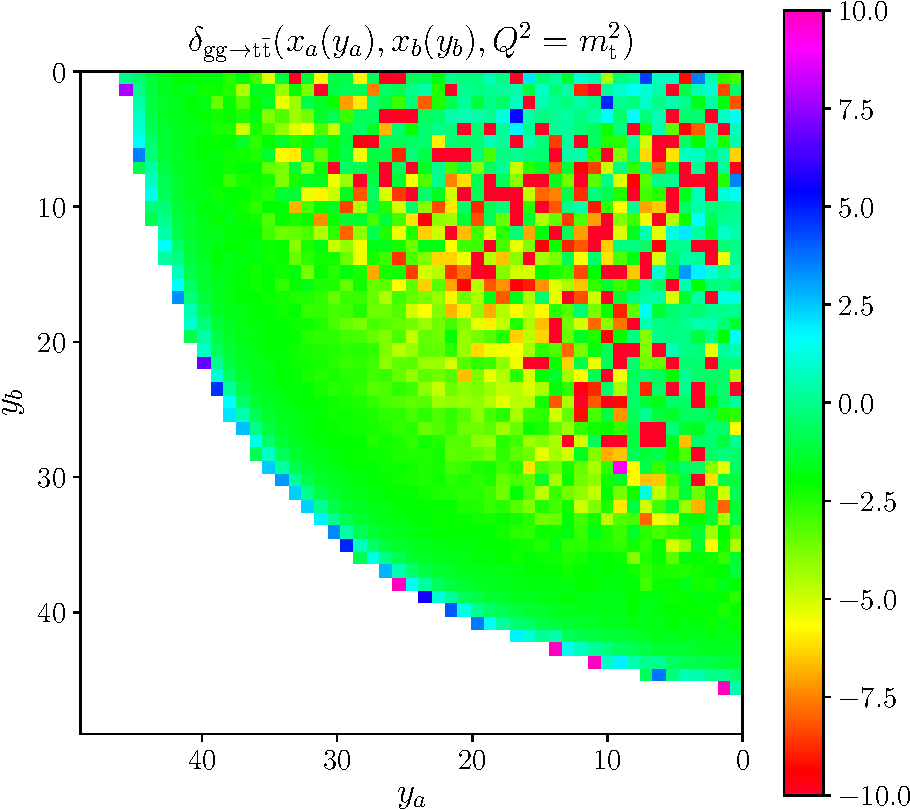
\includegraphics[height=0.73\textheight]{ew_corrections/figures/ttb-crop}
\end{column}
\begin{column}{0.4\textwidth}
\begin{itemize}
\item no interpolation in $y_a$, $y_b$, or $Q^2$
\item correction for ixs roughly \SI{-0.5}{\percent}
\item $y_{a/b}(x) = -\ln x_{a/b} + 5 (1-x_{a/b})$, $y(1) = 0$
\vspace*{0.25cm}
\item lower left corner $\rightarrow$ production threshold
\item at threshold: Coulomb singularity
\item $y_a \leftrightarrow y_b$ symmetry: initial-state symmetry of $\mathrm{g}\mathrm{g} \to \mathrm{t} \bar{\mathrm{t}}$
\item negative correction for larger $x_a$, $x_b$
\end{itemize}
\end{column}
\end{columns}
\end{frame}

\begin{frame}{Interpolation grids (II)}
\fontsize{9}{11}\selectfont
\begin{itemize}
\item Interpolation grids are an old idea:
\begin{itemize}
\item \textrm{\textsc{APPLgrid}} \beamercite{T.\ Carli et al.}{https://inspirehep.net/literature/837019}
\item \textrm{\textsc{fastNLO}} \beamercite{T.\ Kluge, K.\ Rabbertz, M.\ Wobisch}{https://inspirehep.net/literature/727193}
\end{itemize}
\item data generation with
\begin{itemize}
\item \textrm{\textsc{aMCfast}} \beamercite{V.\ Bertone, R.\ Frederix, S.\ Frixione, J.\ Rojo, M.\ Sutton}{https://inspirehep.net/literature/1303899} \\
(\textrm{\textsc{mg5\_aMC@NLO v2+APPLgrid}}) or
\item \textrm{\textsc{MCgrid}} \beamercite{L.D. Debbio, N.P.\ Hartland, S.\ Schuhmann}{https://inspirehep.net/literature/1269460} %\beamercite{E.\ Bothmann, N.P.\ Hartland, S.\ Schuhmann}{https://inspirehep.net/literature/1394617}
(\textrm{\textsc{SHERPA+APPLgrid/fastNLO}})
\item dedicated MCs: \textrm{\textsc{MCFM}}, \textrm{\textsc{NLOjet++}}
\end{itemize}
\item NNPDF uses \textrm{\textsc{APPLgrid}}
\item None of the above support EW corrections
\item \textrm{\textsc{APPLgrid}} is slow and difficult to use; \textrm{\textsc{fastNLO}} has complicated interface
\end{itemize}

\vspace*{\fill}

\begin{itemize}
\item[$\rightarrow$] We wrote \textrm{\textsc{PineAPPL}} (\textrm{\textsc{PineAPPL}} Is Not an Extension of \textrm{\textsc{APPLgrid}})
\item supports arbitrary fixed-order calculations
\item easily supports distributions with more than 1000 bins
\item interfacing with
\begin{itemize}
\item \textrm{\textsc{mg5\_aMC@NLO v3.0.4}} complete, will be released soon
\item \textrm{\textsc{SHERPA+MCgrid}} in progress
\item your custom MC (should be) easily possible!
\end{itemize}
\end{itemize}
\end{frame}

\begin{frame}{\textrm{\textsc{PineAPPL}}}
\fontsize{9}{11}\selectfont
\begin{columns}[T,onlytextwidth]
\begin{column}{.5\textwidth}
\begin{itemize}
\item \beamercite{S.\ Carazza, E.R.\ Nocera, C.\ Schwan, M.\ Zaro}{https://inspirehep.net/literature/1814432}
\item interpolation error typically sub-per mille (see right)
\item off-line PDF uncertainty calculation in a few seconds
\item command-line program to quickly produce predictions
\item simply add: \texttt{set pineappl True} to \texttt{mg5\_aMC} runcard
\item \texttt{C}, \texttt{Python}, \texttt{Rust} interfaces available
\item size of each order, partonic channels, observable
\item support for 1D, 2D, 3D, \ldots, nD distributions
\end{itemize}

\vspace*{0.5cm}

\url{https://n3pdf.github.io/pineappl}
\end{column}
\begin{column}{.5\textwidth}
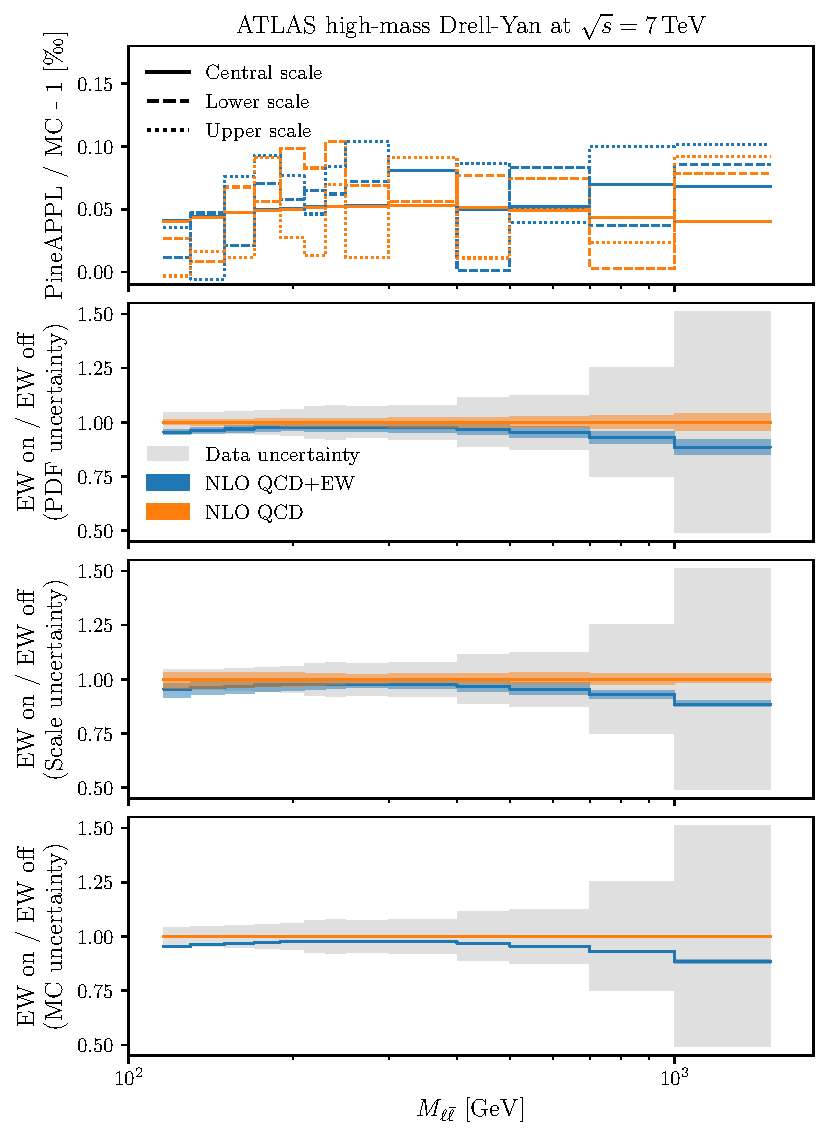
\includegraphics[height=0.89\textheight]{ew_corrections/figures/pineappl_ATLASZHIGHMASS49FB}
\end{column}
\end{columns}
\end{frame}

\begin{frame}{Process list for NNPDF4.0}
\fontsize{9}{11}\selectfont
Calculate theoretical predictions for the entire NNPDF4.0 dataset:
\begin{enumerate}
\item DIS: NMC, SLAC, BCDMS, CHORUS, NUTEV, HERA
\item Fixed-target Drell--Yan experiments
\item Collider experiments (CDF, D{\O}, ATLAS, and CMS)
\begin{itemize}
\item Drell--Yan $\mathrm{Z}$ and $\mathrm{W}^\pm$
\item dijets ATLAS \SI{7}{\tera\electronvolt} and CMS \SIlist{7;8}{\tera\electronvolt} (NEW)
\item single-inclusive jet production ATLAS \SI{8}{\tera\electronvolt} (NEW); peculiar observable,\\
see \beamercite{M.\ Cacciari, S.\ Forte, D.\ Napoletano, G.\ Soyez, G.\ Stagnitto}{https://inspirehep.net/literature/1741988}
\item Top-pair production
\item Z transverse momentum
\item $\mathrm{W}^\pm + \mathrm{c}$ production (at NLO only)
\item W + jets (NEW)
\item single top t-channel production (NEW)
\item diphoton production (NEW)
\end{itemize}
\end{enumerate}

\vspace*{\fill}

\begin{itemize}
\item[$\rightarrow$] for the time being \alert{only collider experiments}; ($N_\text{dat} \approx 1200$)\\
\item[$\rightarrow$] write runcards, validate\\
\item[$\rightarrow$] \alert{explore double-counting issues}, problems with data
\end{itemize}
\end{frame}

\begin{frame}{Drell--Yan: NNPDF4.0 dataset}
\fontsize{9}{11}\selectfont
\begin{columns}[T,onlytextwidth]
\begin{column}{.5\textwidth}

\centering
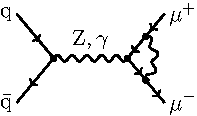
\includegraphics[width=0.32\textwidth]{ew_corrections/figures/fd04_loop_vertex_correction}
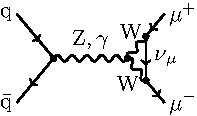
\includegraphics[width=0.32\textwidth]{ew_corrections/figures/fd07_loop_vertex_w_bosons}
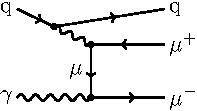
\includegraphics[width=0.32\textwidth]{ew_corrections/figures/fd06_photon_quark_real}

\vspace*{0.4cm}


{\tiny
\begin{center}
\begin{tabular}{@{}l@{~}r@{~}|@{~}l@{~}r@{}}
\toprule
NNPDF ID & $\sqrt{s}$ & NNPDF ID & $\sqrt{s}$ \\
\midrule
\texttt{CDFZRAP} & \SI{1.96}{\tera\electronvolt} & 
\texttt{CMSWEASY840PB} & \SI{7}{\tera\electronvolt} \\
\texttt{D0ZRAP} & \SI{1.96}{\tera\electronvolt} & 
\texttt{CMSWMASY47FB} & \SI{7}{\tera\electronvolt} \\
\texttt{D0WMASY} & \SI{1.96}{\tera\electronvolt} & 
\alert{\texttt{CMSDY2D11}} & \alert{\SI{7}{\tera\electronvolt}} \\
\texttt{ATLASWZRAP36PB} & \SI{7}{\tera\electronvolt} & 
\texttt{CMSWMU8TEV} & \SI{8}{\tera\electronvolt} \\
\texttt{ATLASZHIGHMASS49FB} & \SI{7}{\tera\electronvolt} & 
\texttt{LHCBZ940PB} & \SI{7}{\tera\electronvolt} \\
\texttt{ATLASLOMASSDY11EXT} & \SI{7}{\tera\electronvolt} & 
\texttt{LHCBZEE2FB} & \SI{8}{\tera\electronvolt} \\
\texttt{ATLASWZRAP11CC} & \SI{7}{\tera\electronvolt} & 
\texttt{LHCBWZMU7TEV} & \SI{7}{\tera\electronvolt} \\
\texttt{ATLASWZRAP11CF} & \SI{7}{\tera\electronvolt} & 
\texttt{LHCBWZMU8TEV} & \SI{8}{\tera\electronvolt} \\
\texttt{ATLAS\_DY2D\_8TEV} & \SI{8}{\tera\electronvolt} & 
\texttt{LHCB\_Z\_13TEV\_DIMUON} & \SI{13}{\tera\electronvolt} \\
\texttt{ATLAS\_WZ\_TOT\_13TEV} & \SI{13}{\tera\electronvolt} & 
\texttt{LHCB\_Z\_13TEV\_DIELECTRON} & \SI{13}{\tera\electronvolt} \\
\bottomrule
\end{tabular}
\end{center}
}

\begin{itemize}
\item Observables:
$y_{\ell \bar{\ell}} \approx \frac{1}{2} ln \frac{x_1}{x_2}$ and $M_{\ell \bar{\ell}} \approx \sqrt{x_1 x_2 s}$
\item analysis: \beamercite{CMS Collaboration}{https://inspirehep.net/literature/1262319}
\item NLO EW / NLO QCD: \SI{+11}{\percent} correction, coming from FSR
\end{itemize}

\end{column}
\begin{column}{.5\textwidth}
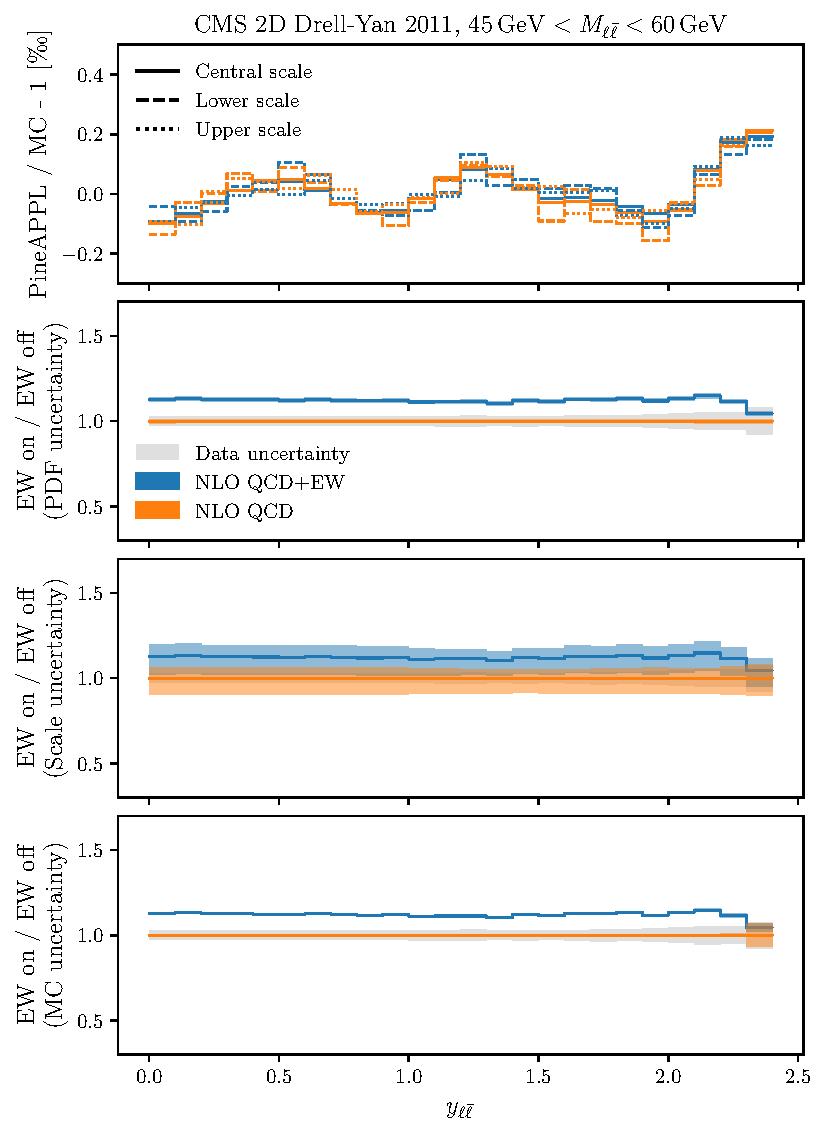
\includegraphics[width=0.94\textwidth]{ew_corrections/figures/pineappl_CMSDY2D11_bin3}
\end{column}
\end{columns}
\end{frame}

\begin{frame}{Double-counting problem: subtraction of FSR}
\fontsize{9}{11}\selectfont
\begin{center}
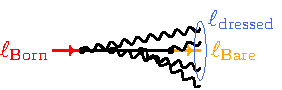
\includegraphics[height=0.2\textheight]{ew_corrections/figures/fd05_photon_radiation}
\end{center}
\begin{itemize}
\item \textcolor{red}{pre-FSR data/Born leptons}: observables of leptons \enquote{before they radiate}, calculated using photon-shower inversion (\textrm{\textsc{PHOTOS}}), from
\item \textcolor{RoyalBlue}{post-FSR data/dressed leptons}: observables using leptons with photons recombined around $\Delta R_{f \gamma}$, typically $\Delta R_{f \gamma} = 0.1$
\end{itemize}
\begin{itemize}
\item \textcolor{red}{pre-FSR data} for comparisons with \textcolor{red}{QCD}-only theory predictions
\item \textcolor{RoyalBlue}{post-FSR data} for comparisons with \textcolor{RoyalBlue}{EW} corrections (up to one photon emission)
\end{itemize}

\vspace*{\fill}

\begin{itemize}
\item Some experiments---notably CMS---do not publish post-FSR data: double counting issue!
\item dressing factors
\begin{equation*}
C_\text{dress} = \frac{\mathrm{d} \sigma_\text{post-FSR} / \mathrm{d} \mathcal{O}}{\mathrm{d} \sigma_\text{pre-FSR} / \mathrm{d} \mathcal{O}}
\end{equation*}
can be large, \alert{up to \SI{20}{\percent}} in invariant mass distributions
\item Often $C_\text{dress}$ (+uncertainty) and pre-FSR dataset given $\Rightarrow$ need to change systematic uncertainties!
\end{itemize}
\end{frame}

\begin{frame}{Subtraction of photon--photon contribution}
\fontsize{9}{11}\selectfont
\begin{center}
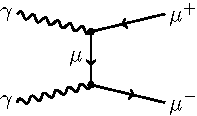
\includegraphics[height=0.2\textheight]{ew_corrections/figures/fd02_born_photon_t_channel}
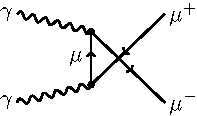
\includegraphics[height=0.2\textheight]{ew_corrections/figures/fd03_born_photon_u_channel}
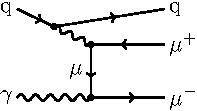
\includegraphics[height=0.2\textheight]{ew_corrections/figures/fd06_photon_quark_real}
\end{center}
\vspace*{\fill}
\begin{itemize}
\item For ATLAS and CMS it seems to be standard procedure to subtract double-photon induced contributions:
\begin{displayquote}
The photon-induced process, $\gamma\gamma \to \ell \bar{\ell}$, is simulated at LO using Pythia 8 and the MRST2004qed PDF set.
\end{displayquote}
\item I am not sure why this is done
\item This is a problem: proton contains photons, should be counted towards signal!
\item Size of the LO contribution can become significant in large-invariant-mass bins (\SI{3}{\percent}) depending on the used PDF---up to twice as large for pre-LUXQED photon PDFs
\end{itemize}
\end{frame}

\begin{frame}[t]{Z transverse momentum}
\fontsize{9}{11}\selectfont
\begin{columns}[T,onlytextwidth]
\begin{column}{.5\textwidth}
\hspace*{1.5cm}
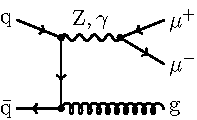
\includegraphics[height=0.13\textheight]{ew_corrections/figures/fd08_z_pt_born}

\vspace*{0.2cm}

\begin{center}
\alert<1>{$\mu = M_\mathrm{Z}$} vs.\ \alert<2>{$\mu = \sqrt{M_\mathrm{Z}^2 + (p_\mathrm{T}^{\ell \bar{\ell}})^2}$}
\end{center}
%\texttt{ATLASZPT8TEVMDIST}
%\texttt{ATLASZPT8TEVYDIST}
%\texttt{ATLAS\_WP\_JET\_8TEV\_PT}
%\texttt{ATLAS\_WM\_JET\_8TEV\_PT}
%\texttt{CMSZDIFF12}
\begin{itemize}
\item FSR issues similar to DY
\item no photon subtraction
\end{itemize}
static scale:
\begin{itemize}
\item accidental cancellation of NLO QCD correction $\rightarrow$ uncertainty band shrinks
\item NLO EW are artificially enhanced because of normalisation
\end{itemize}
dynamic scale:
\begin{itemize}
\item scale variation is stabilised
\item still significant EW corrections, comparable to data uncertainty
\end{itemize}
\end{column}
\begin{column}{.5\textwidth}
\only<1>{\hspace*{\fill}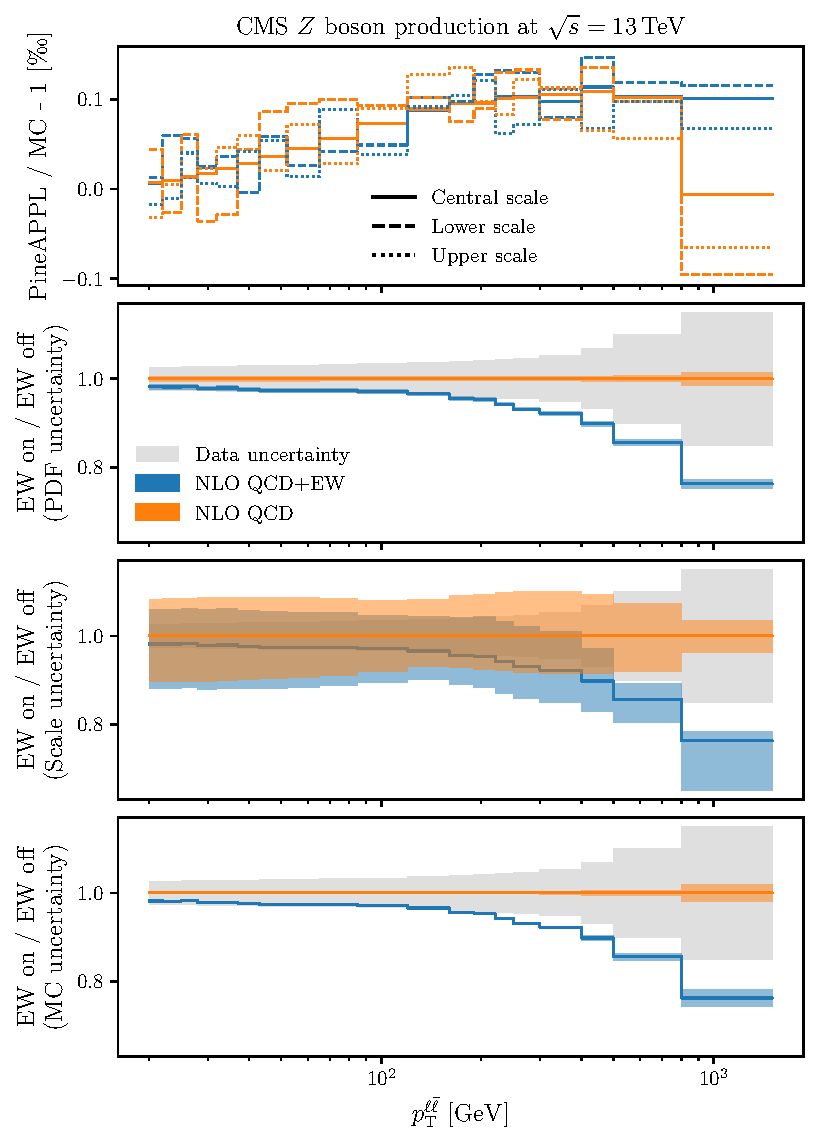
\includegraphics[width=0.9\textwidth]{ew_corrections/figures/pineappl_CMS_Z_13_TEV}}
\only<2>{\hspace*{\fill}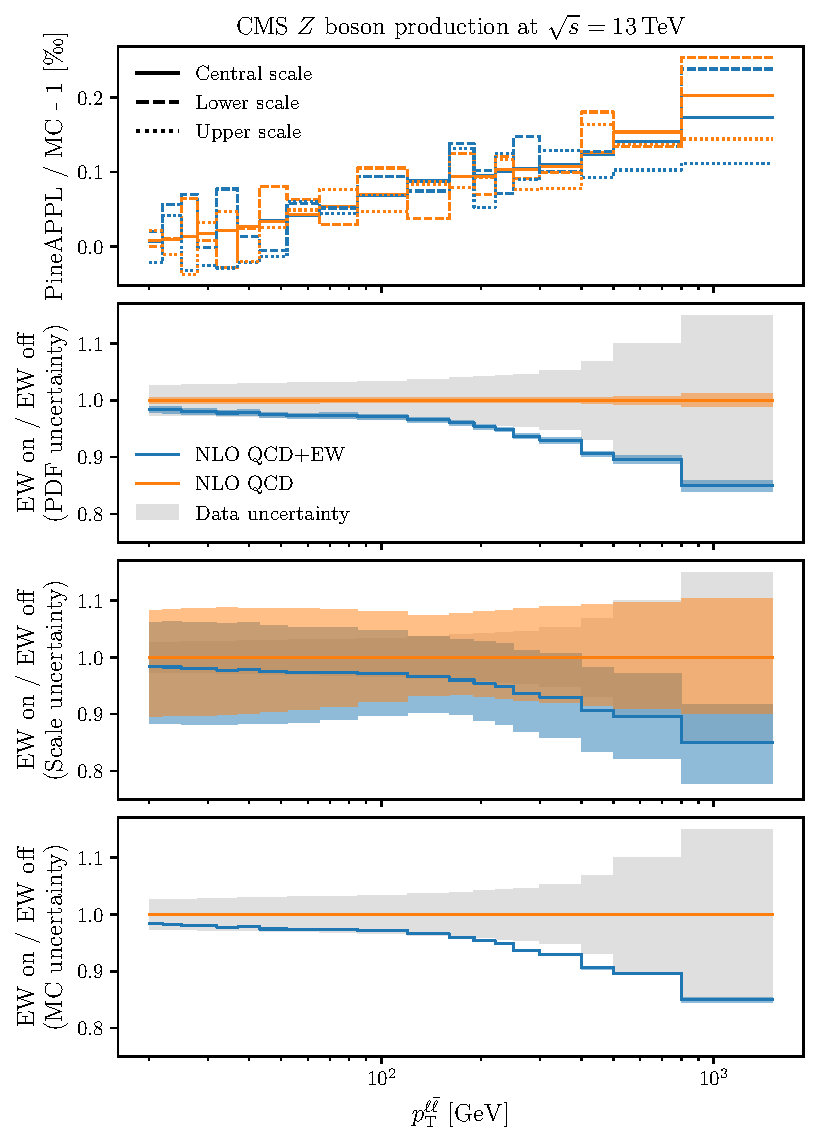
\includegraphics[width=0.9\textwidth]{ew_corrections/figures/pineappl_CMS_Z_13_TEV_dyn}}
\end{column}
\end{columns}
\end{frame}

\begin{frame}{Single-top production}
\fontsize{9}{11}\selectfont
Not properly definable (!?) at NLO EW:
\begin{itemize}
\item Analyses, e.g.\ \beamercite{ATLAS collaboration}{https://inspirehep.net/literature/1303905}, treat $s$-channels as background
\item single-production at LO:
\begin{center}
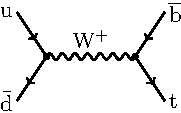
\includegraphics{ew_corrections/figures/fd10_born_s_channel_top}\hspace{0.4cm}
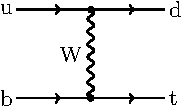
\includegraphics{ew_corrections/figures/fd11_born_t_channel_top}
\end{center}
\item but at NLO EW not (gauge-invariantly) separable:
\begin{center}
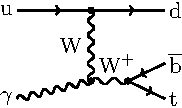
\includegraphics{ew_corrections/figures/fd12_real_ts_channel_top}\hspace{0.4cm}
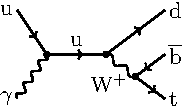
\includegraphics{ew_corrections/figures/fd13_real_s_channel_top}
\end{center}
\item[$\rightarrow$] ignore these datasets?
\item probably not too important, but see \beamercite{E.R.\ Nocera, M.\ Ubiali, C.\ Voisey}{https://inspirehep.net/literature/1772052}
\end{itemize}
\end{frame}

\begin{frame}{\href{https://arxiv.org/abs/1412.1115}{CMS DY 2D} (I)}
\fontsize{9}{11}\selectfont
\begin{columns}
\begin{column}{0.5\textwidth}
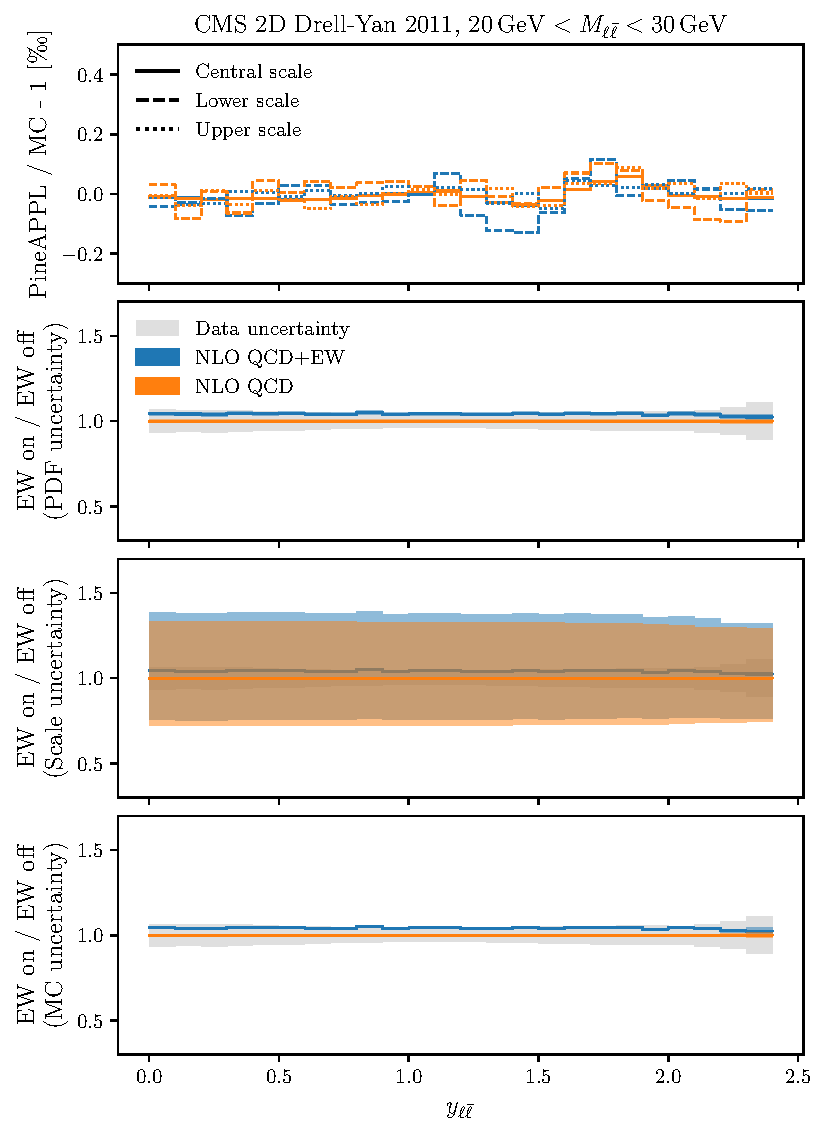
\includegraphics[width=0.95\textwidth]{ew_corrections/figures/pineappl_CMSDY2D11_bin1}
\end{column}
\begin{column}{0.5\textwidth}
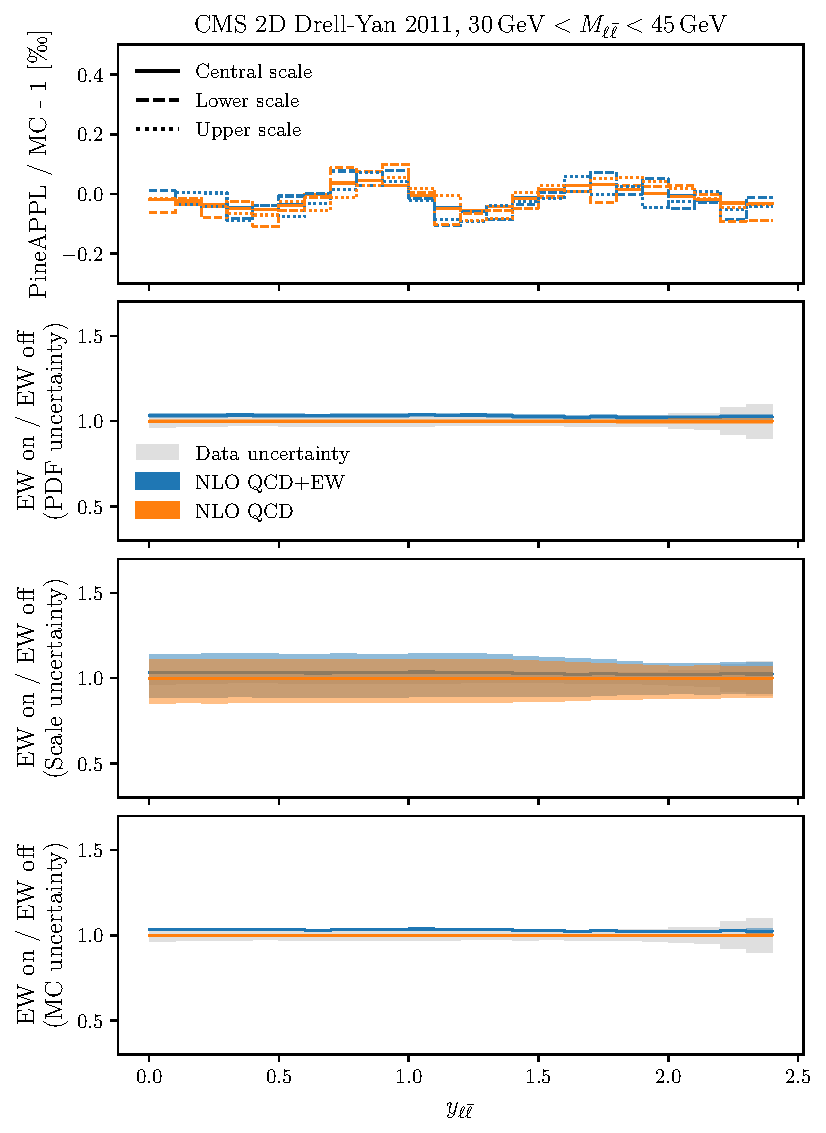
\includegraphics[width=0.95\textwidth]{ew_corrections/figures/pineappl_CMSDY2D11_bin2}
\end{column}
\end{columns}
\end{frame}

\begin{frame}{\href{https://arxiv.org/abs/1412.1115}{CMS DY 2D} (II)}
\fontsize{9}{11}\selectfont
\begin{columns}
\begin{column}{0.5\textwidth}
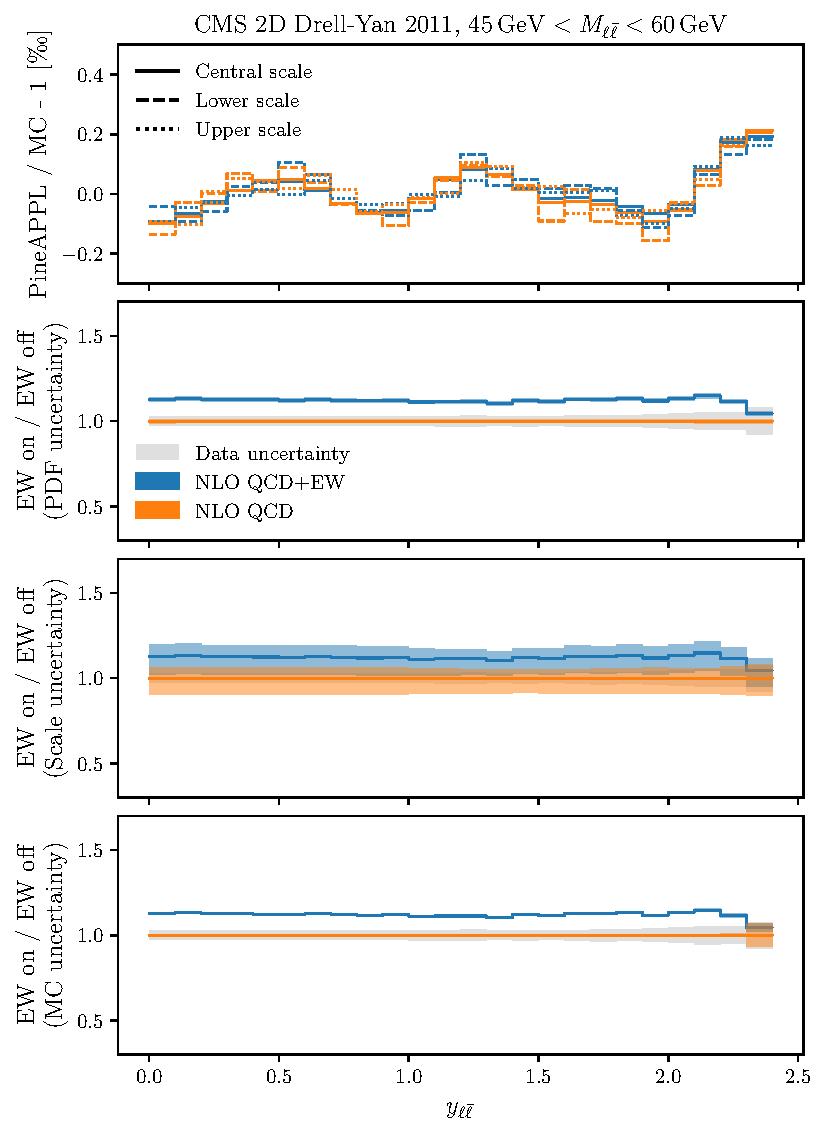
\includegraphics[width=0.95\textwidth]{ew_corrections/figures/pineappl_CMSDY2D11_bin3}
\end{column}
\begin{column}{0.5\textwidth}
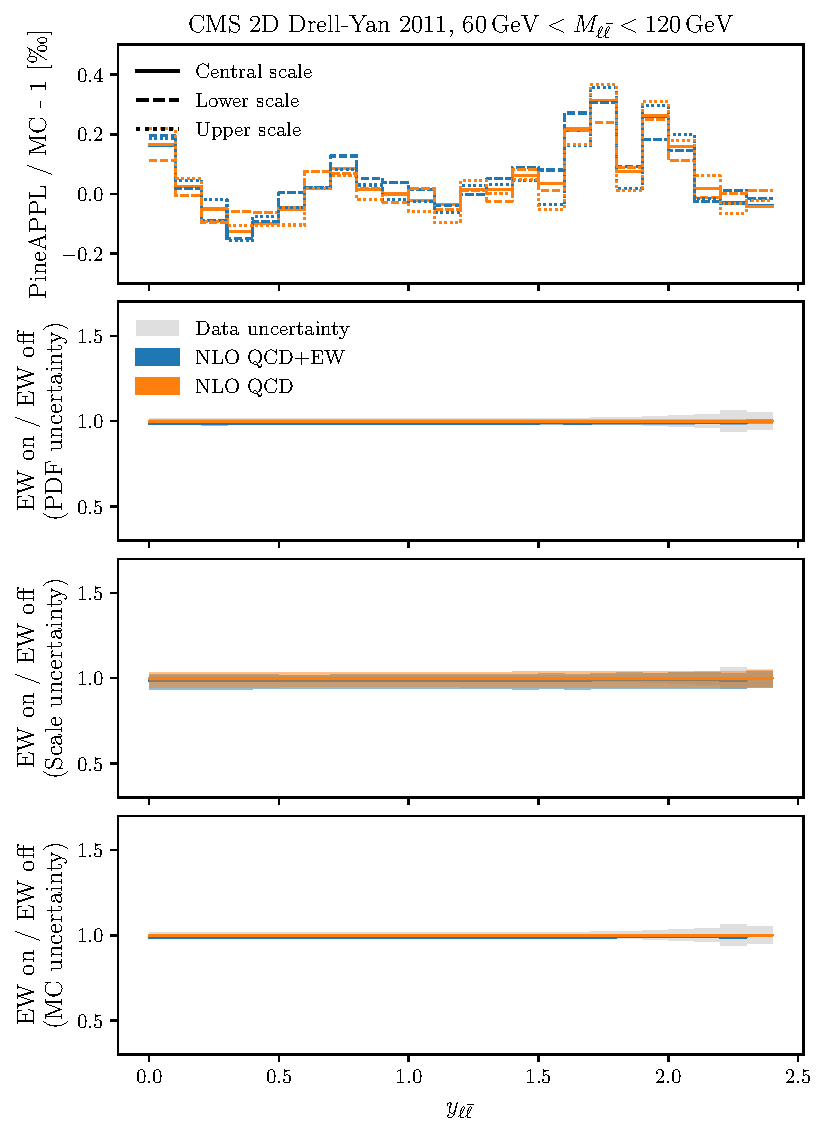
\includegraphics[width=0.95\textwidth]{ew_corrections/figures/pineappl_CMSDY2D11_bin4}
\end{column}
\end{columns}
\end{frame}

\begin{frame}{\href{https://arxiv.org/abs/1412.1115}{CMS DY 2D} (III)}
\fontsize{9}{11}\selectfont
\begin{columns}
\begin{column}{0.5\textwidth}
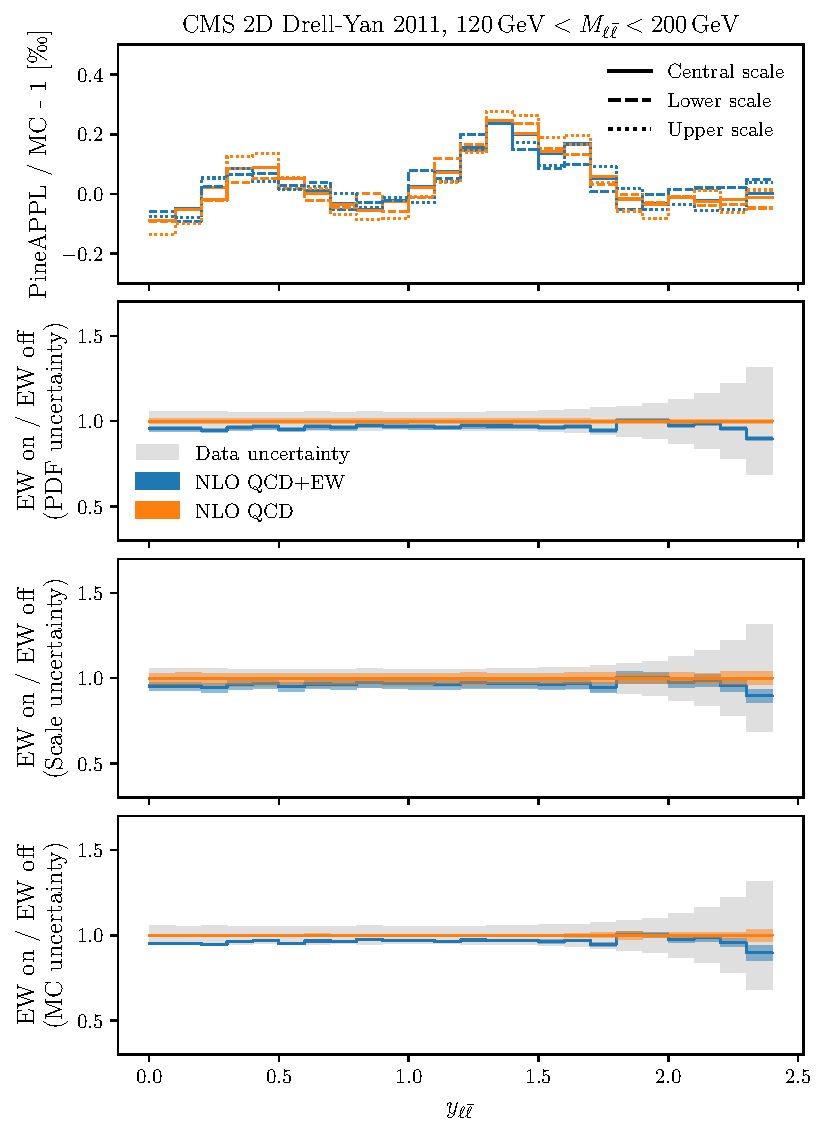
\includegraphics[width=0.95\textwidth]{ew_corrections/figures/pineappl_CMSDY2D11_bin5}
\end{column}
\begin{column}{0.5\textwidth}
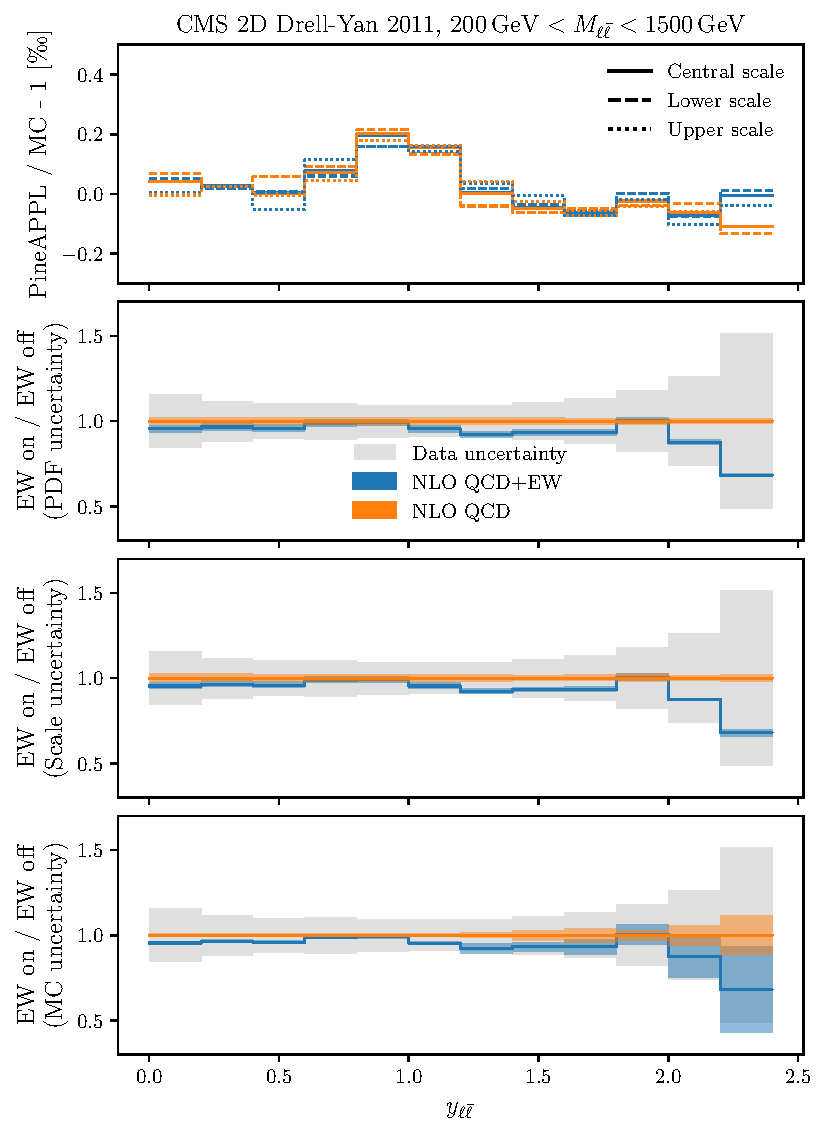
\includegraphics[width=0.95\textwidth]{ew_corrections/figures/pineappl_CMSDY2D11_bin6}
\end{column}
\end{columns}
\end{frame}
